\documentclass[a4paper,12pt]{article}

\usepackage[margin=1in]{geometry}
\usepackage{amsmath,amssymb,amsfonts,amsthm}
\usepackage{mathtools}
\usepackage{tikz}
\setcounter{MaxMatrixCols}{20}
\usepackage{bm}
\usepackage{enumitem}
\usepackage{graphicx}
\usepackage{hyperref}
\usepackage{xcolor}
\usepackage{ascmac}
\usepackage[normalem]{ulem}

\setlength{\parindent}{0pt}
\setlength{\parskip}{0.8em}

\newcommand{\dd}{\,d}
\newcommand{\R}{\mathbb{R}}
\newcommand{\add}[1]{\textcolor{blue}{#1}}
\newcommand{\del}[1]{\textcolor{red}{\sout{#1}}}

\begin{document}
% \pagestyle{plain}

\begin{center}
\begin{large}
\textbf{Homework \#4 ---  MATH 463 (Mathematical Biology)\\
Self-study problems with solutions}
\end{large}\\
\end{center}

\begin{screen}
\begin{itemize}
\item Due 11/12/2026, \textbf{Thursday}, 11:59pm. Submit on Gradescope.
\end{itemize}
\end{screen}

As in the previous homework assignments, I generated this by Claude Opus 5.5, by feeding my section 6 and 7 lecture notes, and then checked and modified it carefully.

Problems 1 and 2 are on section 6 (data-driven discovery of dynamical systems), Problems 3--6 are on section 7 (chemical kinetics), and Problems 7 and 8 are on the first part of section 9 (network biology), that is, pp.~1--8 of those lecture notes.

\begin{enumerate}

\item Self-study \textbf{at least three} of the following problems. At least two of them must come from Problems 1--6. Submit your work, such as hand-written notes or typed notes, as a single pdf (yes, pdf).
\begin{itemize}
\item For other instructions and overarching goals of HW, see the face page of HW1.
\end{itemize}

\end{enumerate}

\textbf{Reminder from section 7.} Michaelis--Menten: for $S + E \xrightleftharpoons[k_{-1}]{k_1} C \xrightarrow{k_2} P + E$, the quasi-steady-state approximation $\frac{\text{d}[C]}{\text{d}t}=0$ together with the conservation law $[E]+[C]=[E_{\text{total}}]$ gives
\[ V = \frac{\text{d}[P]}{\text{d}t} = \frac{V_{\max}[S]}{K_m+[S]},
\qquad V_{\max} = k_2 [E_{\text{total}}],
\qquad K_m = \frac{k_{-1}+k_2}{k_1} . \]
Problem 4(d) asks you to compare your answer with this formula.

\newpage

\section*{Problems}

\subsection*{Problem 1. What SINDy actually does}

Recall the SINDy setup from section 6. We have a time series of $d$ state variables measured at $T$ time points, and we look for
\[ \dot{X} = \Theta(X)\, \Xi . \]

\begin{enumerate}[label=(\alph*)]
\item Say in one sentence each what the three matrices $X$, $\Theta(X)$, and $\Xi$ are, and give the size of each one in terms of $T$, $d$, and $M$ (the number of functions in the library). Which of the three equations do we compute, and which two do we build from the data before we start?

\item Suppose $d=2$, the two state variables are $x$ and $y$, and the library is
\[ \Theta(X) = \begin{bmatrix} 1 & x & y & x^2 & xy & y^2 \end{bmatrix} . \]
SINDy returns
\[
\Xi =
\begin{pmatrix}
0 & 0\\
0.5 & 0\\
0 & -0.3\\
0 & 0\\
-0.1 & 0.05\\
0 & 0
\end{pmatrix},
\]
where the first column is for the $\dot x$ equation and the second column is for the $\dot y$ equation, and the rows are in the order of the library above. Write down the ODE system that SINDy has discovered. Do you recognize it? (We studied it in section 3.)

\item What does the regularization parameter $\alpha$ in
\[ \hat{\Xi} = \underset{\Xi}{\operatorname{argmin}} \left\| \Theta \Xi - \dot{X} \right\|_2 + \alpha \left\| \Xi \right\|_1 \]
control? Describe what you expect to happen to the discovered model if $\alpha$ is taken much too large, and if it is taken much too small.

\item The matrix $\dot X$ is not measured; it has to be computed from the data. Why is this the most dangerous step in practice, and what did Horrocks and Bauch do about it in the epidemic application? (Note: This is not a typical exam question, and I did not teach this directly. However, it is nice to explore.)

\item Suppose that the true dynamics are $\dot x = \frac{x}{1+x} - 0.2x$ (a Michaelis--Menten term, as in section 7), but your library contains only polynomials up to third order. What will SINDy give you? What is the general lesson?
\end{enumerate}

\subsection*{Problem 2. What SINDy cannot determine}

Whether SINDy can determine a model at all depends on how much data we have relative to how large a library we chose, and in this problem we look at why. Throughout, $\dot{X} = \Theta(X)\Xi$ with $X$ of size $T \times d$, $\Theta(X)$ of size $T \times M$, and $\Xi$ of size $M \times d$, as in Problem 1. Take $d=1$ for simplicity, so that $\dot{X}$ is a column vector with $T$ entries and $\Xi$ is a column vector with $M$ entries.

\begin{enumerate}[label=(\alph*)]
\item How many equations and how many unknowns does the linear system $\dot{X}=\Theta\Xi$ have? Answer in terms of $T$ and $M$, and say what each equation and each unknown corresponds to.

\item In linear algebra, what does it mean for a system of linear equations to be overdetermined, and what does it mean for it to be underdetermined? Which of the two is the case here when $T>M$, and which when $T<M$?

\item Explain why the overdetermined case is the situation that we want when we run SINDy on experimental data. (Hint: the measured $\dot{X}$ contains noise. What would it mean to fit it exactly?)

\item Let us see on a small example what goes wrong in the underdetermined case. Take $T=2$ time points and a library of $M=5$ functions,
\[ \Theta(X) = \begin{bmatrix} 1 & x & x^2 & x^3 & x^4 \end{bmatrix} , \]
and suppose that the two measurements are
\[ x\!\left( t_1 \right)=1, \quad \dot{x}\!\left( t_1 \right)=1,
\qquad\qquad
x\!\left( t_2 \right)=2, \quad \dot{x}\!\left( t_2 \right)=8 . \]
\begin{enumerate}[label=(\roman*)]
\item Write down the $2 \times 5$ matrix $\Theta$ and the vector $\dot{X}$ for these data, and say how many equations and how many unknowns the system $\dot{X}=\Theta\Xi$ has.

\item Verify that each of the three models
\[ \dot{x}=x^3, \qquad \dot{x}=-2x+3x^2, \qquad \dot{x}=-6+7x \]
fits both measurements exactly, that is, with a residual of $0$. (Each of them is one choice of $\Xi$; write that $\Xi$ down as well.)

\end{enumerate}

\item In the situation of (d), the fit term $\left\| \Theta\Xi-\dot{X} \right\|_2$ equals $0$ for every one of those infinitely many $\Xi$, so it cannot choose between them. What is the $\ell_1$ term in
\[ \hat{\Xi} = \underset{\Xi}{\operatorname{argmin}} \left\| \Theta \Xi - \dot{X} \right\|_2 + \alpha \left\| \Xi \right\|_1 \]
doing for us in this situation? Compute $\left\| \Xi \right\|_1$ for each of the three models of (d)(ii) to see which one of them the $\ell_1$ term prefers.

\end{enumerate}

\subsection*{Problem 3. A protein that dimerizes}

Many proteins work as \underline{dimers}: two copies of the same molecule $A$ stick together to form $B$. The reaction is reversible:
\[ 2A \xrightleftharpoons[k_{-1}]{k_1} B . \]

\begin{enumerate}[label=(\alph*)]
\item Write down $\frac{\text{d}[A]}{\text{d}t}$ and $\frac{\text{d}[B]}{\text{d}t}$ using the law of mass action. Your equations will contain both a prefactor $2$ and an exponent $2$; explain separately where each of these two $2$'s comes from.

\item Show that $[A] + 2[B]$ does not change in time, and explain what this quantity is. We call it $C$ (the total protein concentration, counted in monomers).

\item At equilibrium, show that $[B] = K [A]^2$, and give $K$ in terms of $k_1$ and $k_{-1}$.

\item Using (b) and (c), show that the equilibrium monomer concentration satisfies
\[ 2K[A]^2 + [A] - C = 0,
\qquad\text{so}\qquad
[A] = \frac{-1+\sqrt{1+8KC}}{4K} . \]
Then, take $K=1$ and compute $[A]$, $[B]$, and the fraction of protein that is in dimers, $\frac{2[B]}{C}$, for $C=1$ and for $C=10$.

\item Show that in the dilute limit $KC \ll 1$ the dimer fraction is approximately $2KC$, so it goes to zero.
\end{enumerate}

\subsection*{Problem 4. A drug that competes with the substrate}

Many drugs work by blocking an enzyme. A \underline{competitive inhibitor} $I$ binds to the same site of the enzyme as the substrate does, so an enzyme molecule that is holding the inhibitor cannot hold the substrate:
\[
S + E \xrightleftharpoons[k_{-1}]{k_1} C \xrightarrow{k_2} P + E,
\qquad
I + E \xrightleftharpoons[k_{-3}]{k_3} C_I .
\]
Here $C_I$ is the enzyme--inhibitor complex, which does nothing else: it cannot make product. Assume that the inhibitor concentration $[I]$ is held fixed.

\begin{enumerate}[label=(\alph*)]
\item Write down the conservation law for the enzyme. (Careful: the enzyme can now be in three states.) (Note: Understand what ``a conservation law'' means first of all.)

\item Apply the quasi-steady-state approximation to $C$, exactly as in the lecture notes. That is, write down $\frac{\text{d}[C]}{\text{d}t}$ by mass action (it has one production term and two loss terms) and set it equal to $0$, and show that
\[ [C] = \frac{[E][S]}{K_m}, \qquad K_m=\frac{k_{-1}+k_2}{k_1} . \]
Do the same for the inhibitor complex: write down $\frac{\text{d}[C_I]}{\text{d}t}$ by mass action, set it equal to $0$, and show that
\[ [C_I] = \frac{[E][I]}{K_I}, \qquad K_I = \frac{k_{-3}}{k_3} . \]

\item Combine (a) and (b) to find $[E]$ in terms of $[S]$ and $[I]$. Then, show that the rate of product formation is
\[ V = \frac{\text{d}[P]}{\text{d}t} = \frac{V_{\max}[S]}{K_m\left( 1 + \frac{[I]}{K_I} \right) + [S]}, \]
where $V_{\max} = k_2 [E_{\text{total}}]$.

\item Compare this with the Michaelis--Menten formula without inhibitor. Which of the two constants, $V_{\max}$ or $K_m$, is changed by the drug, and in which direction?

\item Take $[S] = K_m$. Compute $V/V_{\max}$ without the inhibitor, and with the inhibitor at the concentration $[I] = K_I$.

\item Show that no matter how much inhibitor we add, the rate can always be restored by making $[S]$ large enough. Is this good news or bad news for a drug designer?
\end{enumerate}

\subsection*{Problem 5. How sharp is a Hill curve?}

Here we use the Hill equation from section 7. A protein $P$ binds $n$ molecules of a ligand $S$ at once, all or nothing:
\[ P + nS \xrightleftharpoons[k_{-1}]{k_1} PS . \]
Here $[P]$ is the concentration of the protein with no ligand bound, $[PS]$ is the concentration of the protein with all $n$ ligands bound, and nothing in between exists in this idealized model. The quantity of interest is the fraction of the protein that is carrying ligand,
\[ \theta = \frac{[PS]}{[PS]+[P]} \in [0,1] , \]
which is what an experiment measures (for example, the fraction of hemoglobin that is carrying oxygen). The exponent $n$ is called the Hill coefficient, and the equilibrium constant
\[ K_d = \frac{k_{-1}}{k_1} = \frac{[P][S]^n}{[PS]} \]
is the dissociation constant: a large $K_d$ means that the complex falls apart easily, that is, weak binding. Assume throughout that $[S]$ is held fixed by the environment.

\begin{enumerate}[label=(\alph*)]
\item Derive the Hill equation
\[ \theta = \frac{[S]^n}{[S]^n+K_d} \]
from the equilibrium condition $k_1[P][S]^n = k_{-1}[PS]$ and the definition of $\theta$ above.

\item At which ligand concentration is $\theta = \frac{1}{2}$?

\item Let $[S]_{0.1}$ and $[S]_{0.9}$ be the ligand concentrations at which $\theta = 0.1$ and $\theta = 0.9$. Show that
\[ \frac{[S]_{0.9}}{[S]_{0.1}} = 81^{1/n} . \]
Compute this number for $n=1$ and for $n=4$.

\item Hemoglobin carries oxygen and has $n \approx 2.8$. Using (c), explain in words why cooperative binding ($n>1$) is useful for a molecule that has to pick up oxygen in the lungs and release it in the tissues, where the oxygen concentration is only a few times lower.

\end{enumerate}

\subsection*{Problem 6. A switch made of two enzymes}

A protein $X$ is phosphorylated by a kinase, which converts it into $X_p$, and dephosphorylated back into $X$ by a phosphatase. Each of the two enzymes obeys Michaelis--Menten kinetics, and the lecture notes derived the following equation for this system. The notation is:
\begin{itemize}
\item $X_{\text{total}} = [X]+[X_p]$ is the total amount of the protein, and $y = \frac{[X_p]}{X_{\text{total}}} \in [0,1]$ is the fraction of it that is phosphorylated, so that $1-y$ is the fraction that is not. Only $y$ is needed to describe the state of the system.
\item The kinase acts on the unphosphorylated protein, whose concentration is $[X] = (1-y)X_{\text{total}}$. Its maximal rate is $V_{\max,1}$ and its Michaelis constant is $K_1$.
\item The phosphatase acts on the phosphorylated protein, whose concentration is $[X_p] = y X_{\text{total}}$. Its maximal rate is $V_{\max,2}$ and its Michaelis constant is $K_2$.
\item $J_i = \frac{K_i}{X_{\text{total}}}$ ($i=1,2$) are the two Michaelis constants made dimensionless by the total amount of protein.
\end{itemize}
With this notation,
\[ \frac{\text{d}y}{\text{d}t} = \frac{1}{X_{\text{total}}} \left[ \frac{V_{\max,1}(1-y)}{J_1+1-y} - \frac{V_{\max,2}\,y}{J_2+y} \right] . \]

\begin{enumerate}[label=(\alph*)]
\item Why is it legitimate to treat $X_{\text{total}} = [X]+[X_p]$ as a constant here, even though the cell is constantly making and destroying proteins?

\item Setting $\frac{\text{d}y}{\text{d}t}=0$, show that the steady state $y^*$ satisfies
\[ \frac{V_{\max,1}}{V_{\max,2}} = \frac{y^*\left( J_1+1-y^* \right)}{\left( 1-y^* \right)\left( J_2+y^* \right)} . \]
Note that we have solved for the ratio $\frac{V_{\max,1}}{V_{\max,2}}$ rather than for $y^*$; we will use the formula in this form.

\item Suppose that the two Michaelis constants are small compared with the total amount of protein, that is, $J_1, J_2 \ll 1$. Each enzyme then has far more substrate available than its own Michaelis constant, so each enzyme is \underline{saturated} and works at close to its maximal rate. Show that in this case, for $y$ away from $0$ and $1$,
\[ \frac{\text{d}y}{\text{d}t} \approx \frac{V_{\max,1}-V_{\max,2}}{X_{\text{total}}} , \]
and explain why this makes the steady state a switch: almost all of the protein is phosphorylated if $V_{\max,1}>V_{\max,2}$, and almost none of it is if $V_{\max,1}<V_{\max,2}$.

\item Now add positive feedback: the phosphorylated protein activates its own kinase, so that the kinase activity is proportional to $S+y$, where $S\ge 0$ is an external stimulus. The equation becomes
\[ \frac{\text{d}y}{\text{d}t} = \frac{1}{X_{\text{total}}} \left[ \frac{V_{\max,1}(S+y)(1-y)}{J_1+1-y} - \frac{V_{\max,2}\,y}{J_2+y} \right] . \]
Show that the steady states satisfy
\[ S = \frac{V_{\max,2}}{V_{\max,1}} \cdot \frac{y^*\left( J_1+1-y^* \right)}{\left( 1-y^* \right)\left( J_2+y^* \right)} - y^* . \]

\item Figure~\ref{fig:hw4gk} shows $S$ as a function of $y^*$, computed from the formula in (d) with $J_1=J_2=0.05$ and $V_{\max,1}=V_{\max,2}$.
Using the figure, say how many steady states the system has when $S=0.5$. Which of these steady states are stable and which are unstable? (Hint for the stability: $\frac{\text{d}y}{\text{d}t}$ is a continuous function of the single variable $y$, it is positive at $y=0$ because $S>0$, and it is negative as $y \to 1$.)

\begin{figure}[h]
\begin{center}
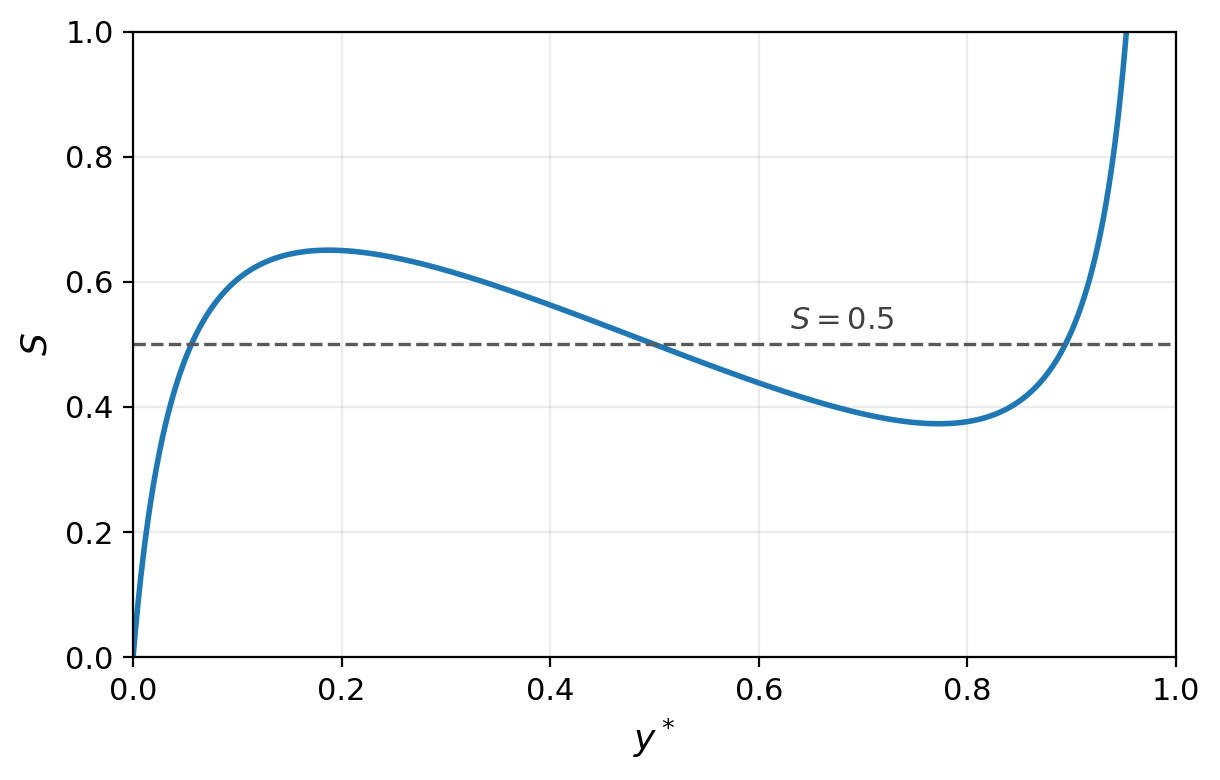
\includegraphics[width=0.72\textwidth]{figures/hw4-gk-feedback.png}
\caption{The stimulus $S$ plotted against the steady state $y^*$, from the formula of Problem 6(d), with $J_1=J_2=0.05$ and $V_{\max,1}=V_{\max,2}$. The dashed line marks $S=0.5$.}
\label{fig:hw4gk}
\end{center}
\end{figure}

\item Using (e), describe what the cell does as the stimulus $S$ is slowly increased from $0$ and then slowly decreased back to $0$. In particular, say where it switches on and where it switches off. This phenomenon is called hysteresis. Which bifurcation occurs at each end of the bistable range?
\end{enumerate}

\subsection*{Problem 7. A small network by hand}

Consider the undirected, unweighted network $G=(V,E)$ with $N=6$ nodes,
\[ V = \left\{ 1,2,3,4,5,6 \right\},
\qquad
E = \Big\{ (1,2),\ (1,3),\ (2,3),\ (3,4),\ (4,5),\ (4,6),\ (5,6) \Big\} . \]

\begin{enumerate}[label=(\alph*)]
\item Draw this network, and write down its $6 \times 6$ adjacency matrix $A$. The network is undirected, is unweighted, and has no self-loops (no edge from a node to itself). State what each of these three facts tells you about $A$.

\item The degree $k_i$ of node $i$ is the number of neighbors that node $i$ has. Show, directly from the definition of the adjacency matrix, that
\[ k_i = \sum_{j=1}^{N} A_{ij} . \]
Compute $k_1, \ldots, k_6$, and write down the degree distribution $p(k)$, that is, the fraction of nodes having degree $k$. Check that $\sum_{k=0}^{N-1} p(k)=1$.

\item Show that in any undirected network without self-loops,
\[ \sum_{i=1}^{N} k_i = 2\left| E \right| , \]
where $\left| E \right|$ is the number of edges, and verify this for our network. Deduce that the average degree is $\left\langle k \right\rangle = \frac{2\left| E \right|}{N}$, and compute it.

\item A \underline{walk of length $2$} from node $i$ to node $j$ is a pair of edges $(i,m)$ and $(m,j)$ for some node $m$; that is, a way of getting from $i$ to $j$ in exactly two hops. Show that the number of such walks equals $\left( A^2 \right)_{ij}$. (Hint: write out $\left( A^2 \right)_{ij} = \sum_{m=1}^{N} A_{im}A_{mj}$ and ask when a term of this sum equals $1$.)

Then compute $\left( A^2 \right)_{14}$ and $\left( A^2 \right)_{15}$ from your drawing.

\item Let $d(i,j)$ be the shortest path length between nodes $i$ and $j$, that is, the number of hops along a shortest path from $i$ to $j$. Using the drawing you made in (a), compute $d(1,4)$ and $d(2,5)$, and in each case give a shortest path that achieves it.

\item Section 9 defines a community (or module) as a densely connected subset of nodes. Which two subsets of nodes would you call the communities of this network, and why?
\end{enumerate}

\subsection*{Problem 8. Small worlds}

The characteristic path length of a network is the average of the shortest path length $d(i,j)$ of Problem 7(e) over all $\frac{N(N-1)}{2}$ unordered pairs of distinct nodes,
\[ L = \frac{2}{N(N-1)}\sum_{i=1}^{N-1}\;\sum_{j=i+1}^{N} d(i,j) . \]
The lecture notes state two facts about it: that $L$ usually grows like $\log N$, which is called the small-world property (in many literature, this is only one of the two conditions to be satisfied for a network to be called small-world though), and that a $d$-dimensional lattice instead gives $L = O\!\left( N^{1/d} \right)$ and so is not a realistic model.

\begin{enumerate}[label=(\alph*)]
\item A ring of $N$ nodes is the one-dimensional lattice: the nodes are arranged on a circle, and each node is joined to its two nearest neighbors. Take $N$ to be even.

Show that the sum of the distances from any one fixed node to the other $N-1$ nodes equals $\frac{N^2}{4}$, and hence that
\[ L = \frac{N^2}{4(N-1)} \approx \frac{N}{4} . \]
Evaluate $L$ for $N=100$ and for $N=1000$.

\item Now consider the square lattice of Figure 3 of the section 9 lecture notes, with $\sqrt{N} \times \sqrt{N}$ nodes, which is the two-dimensional lattice. Roughly how many nodes lie within distance $\ell$ of a given node, when $\ell$ is large but much smaller than $\sqrt{N}$? Use your answer to argue that $L = O\!\left( N^{1/2} \right)$, and then that a $d$-dimensional lattice gives $L = O\!\left( N^{1/d} \right)$. (This question is admittedly rough, good for HW but a bit difficult for me to use in an exam. The solutions provided are correspondingly rough as math (but often favorably used in statistical physics). This is a classical good question that gives you intuition about networks though.)

\item Consider instead a network in which every node has the same degree $k \geq 3$ and which contains no short cycles, so that the neighborhood of any node looks like a tree. Show that the number of nodes at distance exactly $j$ from a given node is $k(k-1)^{j-1}$ for $j \geq 1$, and hence that the number of nodes within distance $\ell$ is
\[ 1 + k\,\frac{(k-1)^{\ell}-1}{k-2} . \]
By setting this equal to $N$, show that
\[ \ell \approx \frac{\log N}{\log (k-1)} , \]
and conclude that $L=O\!\left( \log N \right)$ for such a network.

\item Take $N=10^6$. Compute the estimate of $L$ from (b) with $d=2$, and the estimate from (c) with $k=3$.
(This question is also admittedly rough.)

\end{enumerate}


\newpage

\section*{Solutions}

\subsection*{Solution to Problem 1}

\begin{enumerate}[label=(\alph*)]
\item
\begin{itemize}
\item $X$ is the data matrix: row $t$ is the measured state $\left( x_1(t_t), \ldots, x_d(t_t) \right)$ at the $t$th time point. It is $T \times d$.
\item $\Theta(X)$ is the library: each column is one candidate function (such as $1$, $x$, $x^2$, $xy$, $\sin x$) evaluated along the whole trajectory. It is $T \times M$.
\item $\Xi$ is the coefficient matrix: column $j$ tells us which library functions appear in the equation for $\dot{x}_j$, and with what coefficients. It is $M \times d$.
\end{itemize}
We build $X$ (from the measurements) and $\Theta(X)$ (our choice of candidate functions, evaluated on $X$) before we start, and we also need $\dot{X}$ ($T \times d$), which we estimate from $X$ by numerical differentiation. The unknown that we compute is $\Xi$. The whole point is that $\Xi$ is the only unknown and it enters linearly, which is why a regression can find it.

\item Reading the first column: the entries that are not zero are $0.5$ in the row of $x$ and $-0.1$ in the row of $xy$. Reading the second column: $-0.3$ in the row of $y$ and $0.05$ in the row of $xy$. Therefore
\[
\frac{\text{d}x}{\text{d}t} = 0.5 x - 0.1 xy,
\qquad
\frac{\text{d}y}{\text{d}t} = -0.3 y + 0.05 xy .
\]
This is the Lotka--Volterra predator--prey model from section 3, with $x$ the prey and $y$ the predator.

Note that $4$ of the $12$ entries of $\Xi$ are nonzero. That is what ``sparse'' means here, and it is the reason we can look at the output and recognize a model.

\item The parameter $\alpha$ controls how strongly sparsity is rewarded, that is, how large a penalty we pay for each nonzero coefficient.
\begin{itemize}
\item $\alpha$ much too large: the penalty dominates, and the fit term is almost ignored. Coefficients are driven to zero; in the extreme all of $\Xi$ becomes $0$, that is, $\dot{X}=0$. We get a model that is beautifully simple and wrong (underfitting).
\item $\alpha$ much too small: we are doing ordinary least squares. Every library function gets some small nonzero coefficient, because that is the best way to absorb the noise in $\dot{X}$. The fit to the data is excellent and the output is a dense $\Xi$ that we cannot interpret and that will not generalize (overfitting).
\end{itemize}
So $\alpha$ is a dial between interpretability and goodness of fit, and it has to be chosen, not assumed. Both papers in section 6 choose it (or the equivalent sparsity threshold) by some model selection criterion rather than by eye.

\item Numerical differentiation amplifies noise. If $x(t_t)$ is contaminated by noise of size $\varepsilon$ and the sampling interval is $\Delta t$, then a finite difference $\frac{x(t_{t+1})-x(t_t)}{\Delta t}$ has noise of size $\frac{\varepsilon}{\Delta t}$ or larger. Sampling more finely, which would normally help, makes this worse. And $\dot{X}$ sits on the right-hand side of the regression as the thing we are fitting, so this noise goes straight into $\Xi$: a noisy $\dot{X}$ makes the regression pick up spurious terms in order to chase the noise.

Horrocks and Bauch therefore smoothed the time series before differentiating. The price is that the filter has parameters of its own (window length and polynomial order), and smoothing too aggressively can remove real dynamics along with the noise.

\item A polynomial library cannot represent $\frac{x}{1+x}$ exactly, so SINDy will return the best sparse polynomial approximation. Over a range of small $x$ it would find something like $x - x^2 + \ldots$, which fits well; but it would also happily report coefficients for terms that have no mechanistic meaning, and the model would fail badly outside the range of $x$ covered by the data (a polynomial cannot saturate, whereas $\frac{x}{1+x} \to 1$).

The lesson is that SINDy can only find a model that is in the span of the library you gave it. It is a selection method, not a discovery method in the unlimited sense: the real modeling decision is the choice of library, and that choice requires biological knowledge.
\end{enumerate}

\subsection*{Solution to Problem 2}

\begin{enumerate}[label=(\alph*)]
\item There are $T$ equations and $M$ unknowns.

Each equation corresponds to one time point: row $i$ of the system says that at the $i$th time point $t_i$, the measured derivative must equal the corresponding combination of the library functions evaluated at the measured state,
\[ \dot{x}\!\left( t_i \right) = \sum_{m=1}^{M} \Xi_m \theta_m\!\left( x\!\left( t_i \right) \right) , \]
where $\theta_m$ denotes the $m$th library function. Each unknown $\Xi_m$ is the coefficient of the $m$th library function in the discovered equation, and $\Xi_m=0$ means that function does not appear.

Note that the number of unknowns is set by our choice of library, not by the biology, and the number of equations is set by how much data we have. Both are under our control, which is what parts (b)--(e) are about.

\item A system of linear equations is overdetermined when there are more equations than unknowns, and underdetermined when there are fewer equations than unknowns. An overdetermined system generically has no exact solution at all, so one settles for a best approximate solution, for example the least-squares one. In contrast, an underdetermined system generically has infinitely many exact solutions, so one has to add some other criterion to pick one.

Here the matrix is $\Theta$, of size $T \times M$. So the system is overdetermined when $T>M$, that is, when we have more time points than candidate functions, and underdetermined when $T<M$, that is, when we have more candidate functions than time points.

\item Because the measured $\dot{X}$ contains noise, and we do not want to reproduce the noise.

If the system were solvable exactly, we would obtain a $\Xi$ for which $\Theta\Xi$ equals the measured $\dot{X}$ at every single time point, noise included. But the noise is not part of the dynamics, so such a $\Xi$ is fitting something that carries no information, and the coefficients we would report would be contaminated accordingly. In the overdetermined case, no $\Xi$ can satisfy all $T$ equations, and the least-squares solution is a compromise across all of them. This is the familiar reason for taking many measurements, and the improvement gets better the larger $T$ is relative to $M$. In practice one therefore wants not merely $T>M$ but $T \gg M$.

There is a second reason. An overdetermined system has a unique least-squares solution (when $\Theta$ has full column rank), so the output of the method is well defined: run it twice on the same data and you get the same model.

\item
\begin{enumerate}[label=(\roman*)]
\item Each row of $\Theta$ is the library $\left( 1, x, x^2, x^3, x^4 \right)$ evaluated at one measured state, that is, at $x=1$ and at $x=2$:
\[ \Theta = \begin{pmatrix} 1 & 1 & 1 & 1 & 1\\ 1 & 2 & 4 & 8 & 16 \end{pmatrix},
\qquad
\dot{X} = \begin{pmatrix} 1\\ 8 \end{pmatrix} . \]
The system has $T=2$ equations, one per time point, and $M=5$ unknowns, one per library function. It is underdetermined.

\item Written in the order of the library, the three models are
\[ \Xi = \begin{pmatrix} 0\\ 0\\ 0\\ 1\\ 0 \end{pmatrix},
\qquad
\Xi = \begin{pmatrix} 0\\ -2\\ 3\\ 0\\ 0 \end{pmatrix},
\qquad
\Xi = \begin{pmatrix} -6\\ 7\\ 0\\ 0\\ 0 \end{pmatrix} , \]
and we only have to evaluate each of them at $x=1$ and at $x=2$:
\begin{itemize}
\item $\dot{x}=x^3$: at $x=1$, $1^3=1$ \checkmark; at $x=2$, $2^3=8$ \checkmark.
\item $\dot{x}=-2x+3x^2$: at $x=1$, $-2+3=1$ \checkmark; at $x=2$, $-4+12=8$ \checkmark.
\item $\dot{x}=-6+7x$: at $x=1$, $-6+7=1$ \checkmark; at $x=2$, $-6+14=8$ \checkmark.
\end{itemize}
So all three pass through both data points, and each has a residual of exactly $0$. They are nevertheless completely different dynamical systems: $\dot{x}=x^3$ blows up in finite time, $\dot{x}=-6+7x$ has a steady state at $x=\frac{6}{7}$, and $\dot{x}=-2x+3x^2$ has steady states at $x=0$ and $x=\frac{2}{3}$.

\end{enumerate}

\item In this situation the $\ell_1$ term is the only thing that selects an answer, and what it selects is a solution with a small $\ell_1$ norm.

The reason this is useful is that minimizing $\left\| \Xi \right\|_1$ over a subspace of solutions tends to produce a \underline{sparse} answer, that is, one with many entries exactly equal to zero. (Geometrically: the set $\left\{ \Xi : \left\| \Xi \right\|_1 \leq r \right\}$ is a diamond-shaped ball with corners on the coordinate axes, and as we inflate it from $r=0$ the first point at which it touches the solution subspace is typically one of those corners, where most coordinates vanish.) Sparsity is exactly the property we want, since a sparse $\Xi$ is a short, readable differential equation.

For the three models of (d)(ii),
\[ \left\| \Xi \right\|_1 = 1, \qquad
\left\| \Xi \right\|_1 = \left| -2 \right|+3 = 5, \qquad
\left\| \Xi \right\|_1 = \left| -6 \right|+7 = 13 , \]
respectively, so among the three the $\ell_1$ term prefers $\dot{x}=x^3$ by a wide margin --- and that is the one of the three that uses a single library function. Note that the fit term is blind to this choice, since all three fit perfectly.

(To be honest about the limits of the method: the $\ell_1$ term does not by itself single out one answer here either. For instance $\dot{x}=\frac{8}{15}+\frac{7}{15}x^4$ is also an exact fit and also has $\left\| \Xi \right\|_1 = 1$. What the $\ell_1$ term reliably does is to rule out the dense fits with large coefficients, such as the other two models above.)

\end{enumerate}

\subsection*{Solution to Problem 3}

\begin{enumerate}[label=(\alph*)]
\item The reaction $2A \to B$ is elementary with two molecules of $A$ as reactants, so by mass action its rate is $k_1 [A]^2$; the reverse reaction $B \to 2A$ has rate $k_{-1}[B]$. Each time the forward reaction fires, \underline{two} molecules of $A$ disappear and \underline{one} molecule of $B$ appears. Hence
\[
\frac{\text{d}[A]}{\text{d}t} = -2k_1[A]^2 + 2k_{-1}[B],
\qquad
\frac{\text{d}[B]}{\text{d}t} = k_1[A]^2 - k_{-1}[B] .
\]
The exponent $2$ in $[A]^2$ comes from the rate (two molecules have to meet), whereas the prefactor $2$ comes from the bookkeeping (two molecules are consumed per event). These are two different $2$'s and it is a common mistake to supply one and forget the other.

\item
\[ \frac{\text{d}}{\text{d}t}\left( [A]+2[B] \right) = \left( -2k_1[A]^2+2k_{-1}[B] \right) + 2\left( k_1[A]^2-k_{-1}[B] \right) = 0 . \]
So $[A]+2[B] = C$ is constant. It is the total amount of protein, counted in monomer units: each dimer contains two monomers, hence the factor $2$. The reaction only rearranges monomers into dimers and back; it neither creates nor destroys protein.

Note that $\frac{\text{d}[A]}{\text{d}t} = -2\frac{\text{d}[B]}{\text{d}t}$, which is the same statement.

\item At equilibrium, $\frac{\text{d}[B]}{\text{d}t}=0$ gives $k_1[A]^2 = k_{-1}[B]$, so
\[ [B] = K[A]^2, \qquad K = \frac{k_1}{k_{-1}} . \]
(The same condition makes $\frac{\text{d}[A]}{\text{d}t}=0$, as it must, by (b).) $K$ is an association constant and has units of inverse concentration; its reciprocal $\frac{k_{-1}}{k_1}$ is the dissociation constant.

\item Substituting $[B]=K[A]^2$ into $[A]+2[B]=C$,
\[ [A] + 2K[A]^2 = C, \qquad\text{that is}\qquad 2K[A]^2+[A]-C = 0 . \]
By the quadratic formula,
\[ [A] = \frac{-1 \pm \sqrt{1+8KC}}{4K} . \]
Concentrations are nonnegative, and since $C>0$ we have $\sqrt{1+8KC}>1$, so the $+$ root is the positive one and the $-$ root is negative. Hence
\[ [A] = \frac{-1+\sqrt{1+8KC}}{4K} . \]
Now put $K=1$.
\begin{itemize}
\item $C=1$: $\sqrt{1+8}=3$, so $[A]=\frac{-1+3}{4}=\frac{1}{2}$, $[B]=[A]^2=\frac{1}{4}$, and the dimer fraction is $\frac{2[B]}{C}=\frac{1/2}{1}=\boxed{0.5}$. (Check: $[A]+2[B]=0.5+0.5=1=C$. \checkmark)
\item $C=10$: $\sqrt{1+80}=9$, so $[A]=\frac{-1+9}{4}=2$, $[B]=4$, and the dimer fraction is $\frac{2\cdot 4}{10}=\boxed{0.8}$. (Check: $2+8=10=C$. \checkmark)
\end{itemize}
Note that the dimer fraction is larger at the larger total concentration, $0.8$ against $0.5$. Dimerization is favored by crowding, because two molecules have to meet for the forward reaction to occur (rate $\propto [A]^2$) whereas only one molecule is needed for the reverse (rate $\propto [B]$).

\item For the dilute limit, write $\varepsilon = KC \ll 1$ and expand
\[ \sqrt{1+8\varepsilon} = 1 + 4\varepsilon - 8\varepsilon^2 + O(\varepsilon^3) , \]
so that
\[ [A] = \frac{-1+\sqrt{1+8KC}}{4K} = \frac{4KC-8K^2C^2+O(C^3)}{4K} = C\left( 1 - 2KC \right) + O(C^3) , \]
and therefore
\[ [B] = K[A]^2 = KC^2 + O(C^3),
\qquad
\frac{2[B]}{C} = 2KC + O(C^2) \;\longrightarrow\; 0 . \]
So, in the dilute limit essentially all the protein is monomeric.
\end{enumerate}

\subsection*{Solution to Problem 4}

\begin{enumerate}[label=(\alph*)]
\item An enzyme molecule is either free, or bound to substrate, or bound to inhibitor:
\[ [E] + [C] + [C_I] = [E_{\text{total}}] . \]

\item For $C$, exactly as in the lecture notes,
\[ \begin{aligned}
\frac{\text{d}[C]}{\text{d}t} &= k_1[E][S] - k_{-1}[C] - k_2[C] = 0\\
&\Longrightarrow\quad
[C] = \frac{k_1}{k_{-1}+k_2}[E][S] = \frac{[E][S]}{K_m},
\qquad K_m = \frac{k_{-1}+k_2}{k_1} .
\end{aligned} \]
For $C_I$ there is no catalytic step, so there is one production term and only one loss term:
\[ \frac{\text{d}[C_I]}{\text{d}t} = k_3[E][I] - k_{-3}[C_I] = 0
\quad\Longrightarrow\quad
[C_I] = \frac{k_3}{k_{-3}}[E][I] = \frac{[E][I]}{K_I},
\qquad K_I = \frac{k_{-3}}{k_3} . \]
$K_I$ is the dissociation constant of the inhibitor. A small $K_I$ means tight binding, so a small amount of the drug is enough.

\item Substituting both into (a),
\[ [E]\left( 1 + \frac{[S]}{K_m} + \frac{[I]}{K_I} \right) = [E_{\text{total}}]
\quad\Longrightarrow\quad
[E] = \frac{[E_{\text{total}}]}{1 + \frac{[S]}{K_m} + \frac{[I]}{K_I}} . \]
Then
\[
V = \frac{\text{d}[P]}{\text{d}t} = k_2[C] = \frac{k_2[E][S]}{K_m}
= \frac{k_2[E_{\text{total}}][S]}{K_m\left( 1+\frac{[S]}{K_m}+\frac{[I]}{K_I} \right)}
= \frac{V_{\max}[S]}{K_m\left( 1 + \frac{[I]}{K_I} \right) + [S]} ,
\]
with $V_{\max}=k_2[E_{\text{total}}]$.

\item Writing the result as
\[ V = \frac{V_{\max}[S]}{K_m^{\text{app}} + [S]},
\qquad
K_m^{\text{app}} = K_m\left( 1 + \frac{[I]}{K_I} \right) \geq K_m , \]
we see it is \underline{still} a Michaelis--Menten curve, with
\begin{itemize}
\item $V_{\max}$ unchanged, and
\item $K_m$ increased, by the factor $1+\frac{[I]}{K_I}$.
\end{itemize}
%
% [10/26/2026: I do not fully understand this, so I commented it out. Maybe I can digest it in coming years to be able to include this text back.] This makes sense: a larger $K_m$ means the enzyme behaves as though it had a weaker affinity for the substrate, which is exactly what competition for the same binding site does. And $V_{\max}$ cannot change, because at saturating substrate the substrate wins the competition outright --- every enzyme molecule is holding substrate anyway. (This pair of signatures, $V_{\max}$ fixed and $K_m$ inflated, is how competitive inhibition is identified experimentally, for example as a family of Michaelis--Menten curves with a common asymptote.)

\item At $[S]=K_m$:
\begin{itemize}
\item No inhibitor: $\displaystyle \frac{V}{V_{\max}} = \frac{K_m}{K_m+K_m} = \frac{1}{2}$. (This is the definition of $K_m$: the substrate concentration at half-maximal rate.)
\item $[I]=K_I$: the apparent $K_m$ doubles to $2K_m$, so $\displaystyle \frac{V}{V_{\max}} = \frac{K_m}{2K_m+K_m} = \frac{1}{3} \approx 0.333$.
\end{itemize}

\item For any fixed $[I]$,
\[ \lim_{[S]\to\infty} V = \lim_{[S]\to\infty} \frac{V_{\max}[S]}{K_m^{\text{app}}+[S]} = V_{\max} , \]
so the inhibition can always be overcome by raising the substrate concentration: competitive inhibition is \underline{surmountable}.

For a drug designer this is bad news, and it is a real clinical issue. The substrate concentration in a cell is not under the designer's control, and it may rise --- sometimes in response to the drug itself, since blocking an enzyme causes its substrate to accumulate.
\end{enumerate}

\subsection*{Solution to Problem 5}

\begin{enumerate}[label=(\alph*)]
\item From $k_1[P][S]^n = k_{-1}[PS]$ we get
\[ \frac{[P][S]^n}{[PS]} = \frac{k_{-1}}{k_1} = K_d
\quad\Longrightarrow\quad
[P] = \frac{K_d [PS]}{[S]^n} . \]
Therefore
\[
\theta = \frac{[PS]}{[PS]+[P]}
= \frac{[PS]}{[PS] + \frac{K_d[PS]}{[S]^n}}
= \frac{1}{1+\frac{K_d}{[S]^n}}
= \frac{[S]^n}{[S]^n+K_d} .
\]

\item $\theta=\frac{1}{2}$ requires $[S]^n = K_d$, that is,
\[ [S] = K_d^{1/n} . \]

\item $\theta = \frac{[S]^n}{[S]^n+K_d}$ is equivalent to
\[ \frac{\theta}{1-\theta} = \frac{[S]^n}{K_d}
\qquad\Longrightarrow\qquad
[S]^n = K_d \frac{\theta}{1-\theta} . \]
At $\theta=0.9$, $\frac{\theta}{1-\theta}=9$; at $\theta=0.1$, $\frac{\theta}{1-\theta}=\frac{1}{9}$. Dividing,
\[ \frac{[S]_{0.9}^{\,n}}{[S]_{0.1}^{\,n}} = \frac{9}{1/9} = 81
\qquad\Longrightarrow\qquad
\frac{[S]_{0.9}}{[S]_{0.1}} = 81^{1/n} . \]
\begin{itemize}
\item $n=1$: $81^{1} = \boxed{81}$. We need an \underline{81-fold} change in ligand concentration to go from $10\%$ to $90\%$ bound.
\item $n=4$: $81^{1/4} = \boxed{3}$ exactly, since $81=3^4$. A mere $3$-fold change suffices.
\end{itemize}
This ratio, which is a dimensionless measure of how steep the response is, depends only on $n$ and not on $K_d$: $K_d$ sets where the curve switches, $n$ sets how sharply.

\item For $n=2.8$, $81^{1/2.8} \approx 4.80$: hemoglobin goes from $10\%$ to $90\%$ saturated over a less than $5$-fold change in oxygen concentration, whereas a non-cooperative carrier ($n=1$) would need $81$-fold.

A transport molecule has to do two opposite things: load almost fully where oxygen is plentiful (the lungs) and unload substantially where it is scarce (the tissues). But the oxygen partial pressures at those two places differ only by a factor of a few. With $n=1$ the binding curve is so gradual that over a $3$- to $5$-fold range of oxygen the saturation would barely change: the molecule would arrive in the tissues still mostly loaded and would deliver very little of its cargo. Cooperativity concentrates the whole transition into exactly the narrow concentration window that physiology provides, so that a small drop in oxygen produces a large release. Equivalently, cooperative binding converts a graded chemical signal into a nearly switch-like response.

\end{enumerate}

\subsection*{Solution to Problem 6}

\begin{enumerate}[label=(\alph*)]
\item Because the reactions in this model only interconvert $X$ and $X_p$: phosphorylation moves a molecule from one pool to the other, and dephosphorylation moves it back, so $\frac{\text{d}}{\text{d}t}\left( [X]+[X_p] \right) = 0$. Protein synthesis and degradation do change $X_{\text{total}}$, but they are not part of this model, and the justification is a separation of timescales: phosphorylation and dephosphorylation act on a timescale of seconds, whereas protein synthesis and degradation act on tens of minutes to hours. On the timescale on which the switch operates, $X_{\text{total}}$ has not had time to change appreciably, so it may be treated as a constant parameter. (This is the same kind of reasoning that justifies the quasi-steady-state approximation.)

\item Setting the bracket to zero (the prefactor $\frac{1}{X_{\text{total}}} \neq 0$),
\[ \frac{V_{\max,1}(1-y^*)}{J_1+1-y^*} = \frac{V_{\max,2}\, y^*}{J_2+y^*} . \]
Dividing both sides by $V_{\max,2}$ and by $\frac{1-y^*}{J_1+1-y^*}$,
\[ \frac{V_{\max,1}}{V_{\max,2}} = \frac{y^*}{J_2+y^*} \cdot \frac{J_1+1-y^*}{1-y^*} = \frac{y^*\left( J_1+1-y^* \right)}{\left( 1-y^* \right)\left( J_2+y^* \right)} . \]
It is worth seeing why this form is the useful one. The equation is linear in the ratio $\frac{V_{\max,1}}{V_{\max,2}}$ but quadratic in $y^*$: clearing the denominators to solve for $y^*$ gives a quadratic equation (whose solution is an unpleasant expression involving a square root), whereas the formula above is already in closed form. So instead of asking ``given the enzyme activities, what is $y^*$?'', we ask ``given $y^*$, what enzyme activities would produce it?'', and read the curve backwards. We use this again in (d) and (e).

\item If $J_1 \ll 1$ and $J_1 \ll 1-y$, then $J_1+1-y \approx 1-y$ and so
\[ \frac{V_{\max,1}(1-y)}{J_1+1-y} \approx V_{\max,1} ; \]
similarly, if $J_2 \ll y$, then $\frac{V_{\max,2}\,y}{J_2+y} \approx V_{\max,2}$. Hence, for $y$ bounded away from $0$ and $1$,
\[ \frac{\text{d}y}{\text{d}t} \approx \frac{V_{\max,1}-V_{\max,2}}{X_{\text{total}}} . \]

A constant right-hand side means $y$ moves at a constant speed and cannot stop in the interior. If $V_{\max,1}>V_{\max,2}$, then $\frac{\text{d}y}{\text{d}t}>0$ throughout, so $y$ increases until it gets close enough to $1$ that the approximation $J_1 \ll 1-y$ fails --- which happens only when $1-y = O(J_1)$. The system therefore settles at $y^* \approx 1-O(J_1)$, that is, almost fully phosphorylated. If $V_{\max,1}<V_{\max,2}$, the same argument run backwards gives $y^* = O(J_2)$, almost fully dephosphorylated.

So, the steady state is essentially $0$ or $1$ depending only on the sign of $V_{\max,1}-V_{\max,2}$, creating a step function, i.e., a switch.

\item Setting the bracket to zero again,
\[ \frac{V_{\max,1}(S+y^*)(1-y^*)}{J_1+1-y^*} = \frac{V_{\max,2}\,y^*}{J_2+y^*} , \]
so
\[ S+y^* = \frac{V_{\max,2}}{V_{\max,1}} \cdot \frac{y^*}{J_2+y^*} \cdot \frac{J_1+1-y^*}{1-y^*}
= \frac{V_{\max,2}}{V_{\max,1}} \cdot \frac{y^*\left( J_1+1-y^* \right)}{\left( 1-y^* \right)\left( J_2+y^* \right)} , \]
and therefore
\[ S = \frac{V_{\max,2}}{V_{\max,1}} \cdot \frac{y^*\left( J_1+1-y^* \right)}{\left( 1-y^* \right)\left( J_2+y^* \right)} - y^* . \]

\item The dashed line $S=0.5$ in Figure~\ref{fig:hw4gk} cuts the curve in three places, so for $S=0.5$ the system has three steady states, at approximately
\[ y^* \approx 0.06, \qquad y^* \approx 0.5, \qquad y^* \approx 0.89 . \]
(The middle one is exactly $\frac{1}{2}$ due to a symmetry of this particular case: with $J_1=J_2$ and $V_{\max,1}=V_{\max,2}$ one checks directly that $y^*=\frac{1}{2}$ gives $S=\frac{1}{2}$.)

For the stability, use the hint. The function $\frac{\text{d}y}{\text{d}t}$ is continuous in $y$, it is positive at $y=0$, and it is negative as $y \to 1$, and it vanishes exactly at the three steady states. A continuous function that starts positive, ends negative, and has exactly three zeros must change sign at each of them, so the signs of $\frac{\text{d}y}{\text{d}t}$ on the four intervals are, in order, $+,-,+,-$. Hence $y$ increases toward the lowest steady state from below and decreases toward it from above, and likewise for the highest one, whereas it moves away from the middle one on both sides:
\[ y^* \approx 0.06 \ \text{stable}, \qquad y^*=0.5 \ \text{unstable}, \qquad y^* \approx 0.89 \ \text{stable}. \]
The system is bistable.

\item Read Figure~\ref{fig:hw4gk} sideways, that is, as a graph of $y^*$ against $S$ rather than of $S$ against $y^*$. We obtain an S-shaped (``sideways S'') curve with a lower branch, an unstable middle branch, and an upper branch.

First consider increasing $S$ from $0$. At $S=0$ the only steady state is $y^*=0$ (unphosphorylated, switch off), and as $S$ increases the state tracks the lower branch, with $y^*$ rising slowly and staying small. Nothing dramatic happens as we pass $S \approx 0.37$, where the upper (stable) branch comes into existence; the cell stays on the lower branch, because it is stable and the cell is already sitting on it. But when $S$ exceeds the local maximum, $S \approx 0.65$, the lower branch and the middle (unstable) branch collide and annihilate. There is now nothing left for the system to sit on near $y \approx 0.19$, so $y$ shoots up to the only remaining steady state, on the upper branch at $y^* \approx 0.92$: the switch turns on abruptly.

Now consider decreasing $S$ back to $0$. The system is now on the upper branch and stays there. At $S \approx 0.65$, where it jumped up, nothing happens --- it does not jump back. It keeps tracking the upper branch down until $S$ falls below the local minimum, $S \approx 0.37$, at which the upper branch collides with the middle branch and disappears (this happens at $y \approx 0.77$), and $y$ drops back to the lower branch, to $y^* \approx 0.03$: the switch turns off, but at a different value of $S$ from where it turned on.
This is hysteresis.

At each end of the bistable range, two steady states (one stable, one unstable) collide and annihilate as the parameter crosses a critical value. From section 3, this is a saddle-node bifurcation. There is a saddle-node bifurcation at $S \approx 0.651$ and another at $S \approx 0.373$.
\end{enumerate}

\subsection*{Solution to Problem 7}

\begin{enumerate}[label=(\alph*)]
\item Nodes $1,2,3$ form a triangle, nodes $4,5,6$ form another triangle, and the single edge $(3,4)$ joins the two:
\begin{center}
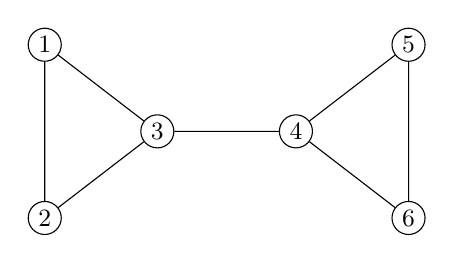
\begin{tikzpicture}[scale=1.1,every node/.style={circle,draw,inner sep=1.6pt,font=\small}]
\node (n1) at (0,1) {1};
\node (n2) at (0,-1) {2};
\node (n3) at (1.3,0) {3};
\node (n4) at (2.9,0) {4};
\node (n5) at (4.2,1) {5};
\node (n6) at (4.2,-1) {6};
\draw (n1)--(n2) (n1)--(n3) (n2)--(n3) (n3)--(n4) (n4)--(n5) (n4)--(n6) (n5)--(n6);
\end{tikzpicture}
\end{center}
The adjacency matrix, with the rows and columns in the order $1,2,3,4,5,6$, is
\[ A = \begin{pmatrix}
0 & 1 & 1 & 0 & 0 & 0\\
1 & 0 & 1 & 0 & 0 & 0\\
1 & 1 & 0 & 1 & 0 & 0\\
0 & 0 & 1 & 0 & 1 & 1\\
0 & 0 & 0 & 1 & 0 & 1\\
0 & 0 & 0 & 1 & 1 & 0
\end{pmatrix} . \]
The three facts correspond to three properties of $A$:
\begin{itemize}
\item Undirected: the edge $(i,j)$ is the same object as the edge $(j,i)$, so $A_{ij}=A_{ji}$, that is, $A$ is symmetric.
\item Unweighted: every entry is $0$ or $1$, rather than an arbitrary nonnegative weight.
\item No self-loops: $A_{ii}=0$ for all $i$, that is, the diagonal is zero.
\end{itemize}

\item By definition $A_{ij}=1$ exactly when $j$ is a neighbor of $i$, and $A_{ij}=0$ otherwise. So the sum $\sum_{j=1}^{N} A_{ij}$ adds $1$ once for each neighbor of $i$ and $0$ for every other node, which is precisely the number of neighbors of $i$:
\[ \sum_{j=1}^{N} A_{ij} = k_i . \]
In other words, the degree of node $i$ is the sum of the $i$th row of $A$ (and, by symmetry, of the $i$th column).

Summing the rows above,
\[ k_1=2, \quad k_2=2, \quad k_3=3, \quad k_4=3, \quad k_5=2, \quad k_6=2 . \]
Four of the six nodes have degree $2$ and two of them have degree $3$, so
\[ p(2)=\frac{4}{6}=\frac{2}{3}, \qquad p(3)=\frac{2}{6}=\frac{1}{3}, \qquad p(k)=0 \ \text{ otherwise} , \]
or, in the notation used in the lecture notes, $p(k) = \frac{2}{3}\delta_{k,2}+\frac{1}{3}\delta_{k,3}$.

\item Count the quantity $\sum_{i=1}^{N} k_i$ in a different way. By (b), $\sum_{i=1}^{N} k_i = \sum_{i=1}^{N} \sum_{j=1}^{N} A_{ij}$, which is the sum of all the entries of $A$. Each edge $(i,j)$ of the network contributes exactly two entries equal to $1$ to this sum, namely $A_{ij}$ and $A_{ji}$. Therefore,
\[ \sum_{i=1}^{N} k_i = 2\left| E \right| . \]
(Equivalently: each edge has two endpoints, and summing the degrees counts each edge once at each of its two endpoints.)

Here $\left| E \right| = 7$ and $\sum_{i=1}^{N} k_i = 2+2+3+3+2+2 = 14 = 2 \times 7$. \checkmark

For the average degree,
\[ \left\langle k \right\rangle = \sum_{k=0}^{N-1} k\,p(k) = \frac{1}{N}\sum_{i=1}^{N} k_i = \frac{2\left| E \right|}{N} , \]
where the middle expression is just the definition of an average over the nodes and the last step uses the identity above. Numerically,
\[ \left\langle k \right\rangle = \frac{14}{6} = \frac{7}{3} \approx 2.33 . \]

\item We have
\[ \left( A^2 \right)_{ij} = \sum_{m=1}^{N} A_{im}A_{mj} . \]
Each term of this sum is $0$ or $1$, and $A_{im}A_{mj}=1$ holds exactly when $A_{im}=1$ and $A_{mj}=1$, that is, exactly when $m$ is adjacent to $i$ and also adjacent to $j$ --- which is exactly when $(i,m)$ and $(m,j)$ is a walk of length $2$ from $i$ to $j$. So the sum counts the intermediate nodes $m$ that give such a walk, one for each walk. Hence $\left( A^2 \right)_{ij}$ is the number of walks of length $2$ from $i$ to $j$, and for $i \neq j$ this is the number of common neighbors of $i$ and $j$.

From the drawing: the neighbors of node $1$ are $\{2,3\}$ and the neighbors of node $4$ are $\{3,5,6\}$, whose only common element is node $3$, so
\[ \left( A^2 \right)_{14} = 1 \qquad\text{(the walk } 1-3-4 \text{)} . \]
The neighbors of node $5$ are $\{4,6\}$, which has no element in common with $\{2,3\}$, so
\[ \left( A^2 \right)_{15} = 0 . \]

\item From the drawing, every route out of the left-hand triangle $\{1,2,3\}$ has to use the bridge $(3,4)$, so a shortest path from node $1$ to anything on the right must first reach node $3$.

For $d(1,4)$: node $1$ is not adjacent to node $4$, so $d(1,4)>1$; and $1-3-4$ is a route of two hops. Hence
\[ d(1,4)=2, \qquad\text{along } 1-3-4 . \]
For $d(2,5)$: node $2$ is adjacent only to $1$ and $3$, neither of which is adjacent to node $5$, so there is no route of one or two hops and $d(2,5)>2$; and $2-3-4-5$ is a route of three hops. Hence
\[ d(2,5)=3, \qquad\text{along } 2-3-4-5 . \]
In general a shortest path need not be unique, and only its length $d(i,j)$ is well defined.

\item The communities are
\[ \left\{ 1,2,3 \right\} \qquad\text{and}\qquad \left\{ 4,5,6 \right\} . \]
Each of these three-node subsets is as densely connected as it possibly could be: all $3$ of the possible edges within it are present, so each is a triangle. Between the two subsets, by contrast, there are $3 \times 3 = 9$ possible edges and only $1$ is present. Densely connected inside, sparsely connected to the outside, is exactly the notion of a community in a network.

\end{enumerate}

\subsection*{Solution to Problem 8}

\begin{enumerate}[label=(\alph*)]
\item Fix a node and label the others by how far around the circle they are. Going clockwise we meet nodes at distances $1,2,\ldots$ and going counterclockwise likewise, and the node diametrically opposite is reached at distance $\frac{N}{2}$ either way. So, with $N$ even, the multiset of distances from our fixed node consists of each of $1,2,\ldots,\frac{N}{2}-1$ exactly twice, together with $\frac{N}{2}$ once. That accounts for $2\left( \frac{N}{2}-1 \right)+1 = N-1$ nodes, as it should. Therefore
\[ \sum_{\substack{j=1 \\ j \neq i}}^{N} d(i,j)
= 2\sum_{m=1}^{\frac{N}{2}-1} m + \frac{N}{2}
= 2 \cdot \frac{\left( \frac{N}{2}-1 \right)\frac{N}{2}}{2} + \frac{N}{2}
= \frac{N}{2}\left( \frac{N}{2}-1 \right) + \frac{N}{2}
= \frac{N}{2} \cdot \frac{N}{2}
= \frac{N^2}{4} . \]
By the symmetry of the ring this sum is the same for every choice of the fixed node, so summing over all $N$ choices counts every ordered pair once:
\[ L = \frac{1}{N(N-1)}\sum_{i=1}^{N}\;\sum_{\substack{j=1 \\ j \neq i}}^{N} d(i,j) = \frac{1}{N(N-1)} \cdot N \cdot \frac{N^2}{4} = \frac{N^2}{4(N-1)} \approx \frac{N}{4} . \]
Numerically,
\[ N=100: \quad L = \frac{10^4}{396} = 25.3 ,
\qquad\qquad
N=1000: \quad L = \frac{10^6}{3996} = 250.3 . \]
Multiplying $N$ by $10$ multiplies $L$ by $10$: the growth is linear in $N$, which is $O\!\left( N^{1/d} \right)$ with $d=1$.

\item On the square lattice, the set of nodes within distance $\ell$ of a given node is a diamond-shaped region (a ball in the Manhattan metric) of radius $\ell$; see Figure~\ref{fig:hw4lattice}. The nodes at distance exactly $m$ are the lattice points on the boundary of the diamond of radius $m$, and there are $4m$ of them: that boundary has four straight sides, each carrying $m$ of those nodes if we count one endpoint of each side and not the other. Hence the number of nodes within distance $\ell$ is
\[ 1+\sum_{m=1}^{\ell} 4m = 2\ell^2+2\ell+1 \approx 2\ell^2 ; \]
the point is simply that it is of order $\ell^2$, because the region is two-dimensional and its area grows like the square of its radius. In $d$ dimensions the corresponding count is of order $\ell^d$.

\begin{figure}[h]
\begin{center}
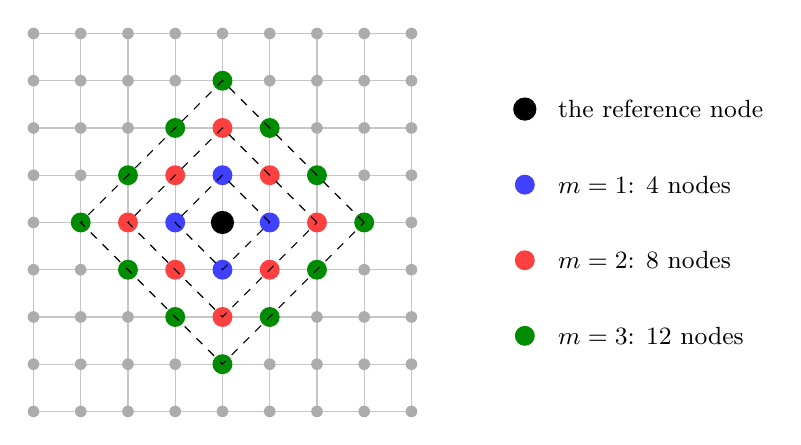
\begin{tikzpicture}[scale=0.6]
\foreach \i in {-4,...,4} {
  \draw[gray!45] (\i,-4)--(\i,4);
  \draw[gray!45] (-4,\i)--(4,\i);
}
\foreach \i in {-4,...,4} {
  \foreach \j in {-4,...,4} {
    \pgfmathtruncatemacro{\dist}{abs(\i)+abs(\j)}
    \ifnum\dist=0 \fill[black] (\i,\j) circle (7pt); \fi
    \ifnum\dist=1 \fill[blue!75] (\i,\j) circle (6pt); \fi
    \ifnum\dist=2 \fill[red!75] (\i,\j) circle (6pt); \fi
    \ifnum\dist=3 \fill[green!55!black] (\i,\j) circle (6pt); \fi
    \ifnum\dist>3 \fill[gray!65] (\i,\j) circle (3.5pt); \fi
  }
}
\foreach \m in {1,2,3} {
  \draw[dashed] (\m,0)--(0,\m)--(-\m,0)--(0,-\m)--cycle;
}
\fill[black] (6.4,2.4) circle (7pt);
\node[right,font=\small] at (6.9,2.4) {the reference node};
\fill[blue!75] (6.4,0.8) circle (6pt);
\node[right,font=\small] at (6.9,0.8) {$m=1$: $4$ nodes};
\fill[red!75] (6.4,-0.8) circle (6pt);
\node[right,font=\small] at (6.9,-0.8) {$m=2$: $8$ nodes};
\fill[green!55!black] (6.4,-2.4) circle (6pt);
\node[right,font=\small] at (6.9,-2.4) {$m=3$: $12$ nodes};
\end{tikzpicture}
\caption{Counting nodes on the square lattice. The nodes at distance $m$ from the reference node lie on the dashed diamond of radius $m$, and there are $4m$ of them. The ball of radius $\ell=3$ therefore holds $1+4+8+12=25$ nodes, which is of order $\ell^2$.}
\label{fig:hw4lattice}
\end{center}
\end{figure}

Now, most of the other $N-1$ nodes have to be within distance $L$ of our node, more or less by the definition of the average. So we need the ball of radius of order $L$ to contain of order $N$ nodes:
\[ c\,L^d \sim N \qquad\Longrightarrow\qquad L \sim \left( \frac{N}{c} \right)^{1/d} = O\!\left( N^{1/d} \right) . \]
For $d=2$ this gives $L = O\!\left( N^{1/2} \right)$, and $d=1$ recovers the answer of part (a).

\item Start at a node and walk outward; Figure~\ref{fig:hw4tree} shows the first three steps for $k=3$. Our starting node has $k$ neighbors, so there are $k$ nodes at distance $1$. Take any one of them: it has $k$ edges, one of which leads back to the starting node, so it has $k-1$ edges leading onward, giving $k(k-1)$ nodes at distance $2$. Because there are no short cycles, no two of these onward edges lead to the same node, and none leads back into a node we have already counted; so the count multiplies by $k-1$ at every further step, and the number of nodes at distance exactly $j$ is
\[ k(k-1)^{j-1} \qquad (j \geq 1) . \]

\begin{figure}[h]
\begin{center}
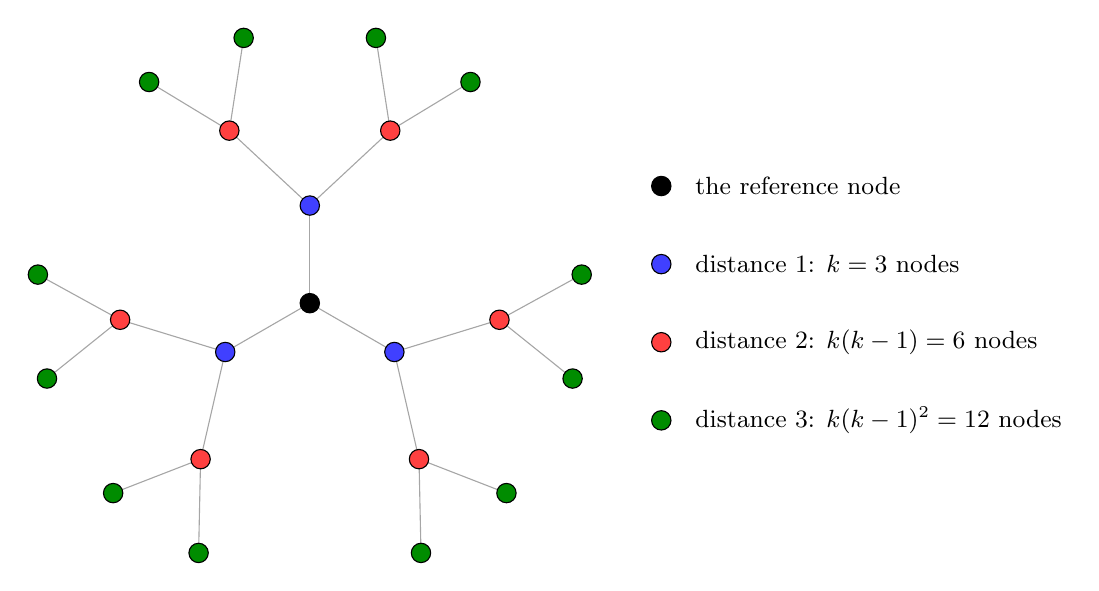
\begin{tikzpicture}[scale=0.62,
  nd/.style={circle,draw,inner sep=0pt,minimum size=7pt}]
\def\ra{2.0}
\def\rb{3.9}
\def\rc{5.6}
\foreach \a in {90,210,330} { \draw[gray!70] (0,0)--(\a:\ra); }
\foreach \a/\b in {90/65,90/115,210/185,210/235,330/305,330/355}
  { \draw[gray!70] (\a:\ra)--(\b:\rb); }
\foreach \b/\c in {65/54,65/76,115/104,115/126,185/174,185/196,235/224,235/246,305/294,305/316,355/344,355/6}
  { \draw[gray!70] (\b:\rb)--(\c:\rc); }
\node[nd,fill=black] at (0,0) {};
\foreach \a in {90,210,330} { \node[nd,fill=blue!75] at (\a:\ra) {}; }
\foreach \b in {65,115,185,235,305,355} { \node[nd,fill=red!75] at (\b:\rb) {}; }
\foreach \c in {6,54,76,104,126,174,196,224,246,294,316,344} { \node[nd,fill=green!55!black] at (\c:\rc) {}; }
\node[nd,fill=black] at (7.2,2.4) {};
\node[right,font=\small] at (7.7,2.4) {the reference node};
\node[nd,fill=blue!75] at (7.2,0.8) {};
\node[right,font=\small] at (7.7,0.8) {distance $1$: $k=3$ nodes};
\node[nd,fill=red!75] at (7.2,-0.8) {};
\node[right,font=\small] at (7.7,-0.8) {distance $2$: $k(k-1)=6$ nodes};
\node[nd,fill=green!55!black] at (7.2,-2.4) {};
\node[right,font=\small] at (7.7,-2.4) {distance $3$: $k(k-1)^2=12$ nodes};
\end{tikzpicture}
\caption{Counting nodes in a network in which every node has degree $k=3$ and the neighborhood of a node contains no cycle. The count is multiplied by $k-1=2$, and not by $k$, at each step outward, because one of the $k$ edges of each node is the one we arrived along.}
\label{fig:hw4tree}
\end{center}
\end{figure}
Summing the geometric series, the number of nodes within distance $\ell$ (including the starting node itself) is
\[ 1+\sum_{j=1}^{\ell} k(k-1)^{j-1}
= 1 + k\,\frac{(k-1)^{\ell}-1}{(k-1)-1}
= 1+k\,\frac{(k-1)^{\ell}-1}{k-2} , \]
where we used $\sum_{j=1}^{\ell} r^{j-1} = \frac{r^{\ell}-1}{r-1}$ with $r=k-1 \neq 1$, which is where $k \geq 3$ is needed.

Setting this equal to $N$ and keeping only the dominant term for large $\ell$,
\[ \begin{aligned}
\frac{k}{k-2}(k-1)^{\ell} &\approx N\\
\Longrightarrow\quad \ell \log(k-1) &\approx \log N + \log\frac{k-2}{k}\\
\Longrightarrow\quad \ell &\approx \frac{\log N}{\log (k-1)} ,
\end{aligned} \]
the neglected term being a constant independent of $N$. Since essentially all of the network is reached within this many hops, the typical distance is of this order, so
\[ L = O\!\left( \log N \right) . \]
The contrast with (b) is the whole point: here the number of nodes reachable in $\ell$ hops grows exponentially in $\ell$, rather than polynomially, because there is no space to be confined to. Exponential growth outward is the same thing as logarithmic distances.

\item With $N=10^6$:
\begin{itemize}
\item From (b) with $d=2$: $L \sim N^{1/2} = 10^3$. (A more careful calculation of the average Manhattan distance on a $1000 \times 1000$ grid gives $L \approx \frac{2}{3}\sqrt{N} \approx 667$, which is the same order of magnitude.)
\item From (c) with $k=3$: $\ell \approx \frac{\log 10^6}{\log 2} = \frac{13.82}{0.693} \approx 20$. (Solving $3 \cdot 2^{\ell}-2 = 10^6$ exactly gives $\ell = 18.3$, so about $19$ hops; again the same answer.)
\end{itemize}
The two estimates differ by a factor of about $50$: in the lattice two nodes of a million are typically a thousand steps apart, whereas in the tree-like network they are about $20$ steps apart.

\end{enumerate}

\end{document}
